\documentclass[10pt, unicode]{beamer}
\usepackage{fontspec}
\usepackage{polyglossia}
\setdefaultlanguage{english}
\usepackage{graphics}
\usepackage{graphicx}
\usepackage{subcaption}
\usepackage{float}
\usepackage{caption}
\usepackage{newfloat}

\graphicspath{{images/}}

\DeclareMathOperator{\sech}{sech}
\setsansfont{Fira Sans}
\title{Генерация текстурного меша и упаковка полигональных текстур в атлас}
\author[Терехов Д.Е.]{Студент группы Б8403а Терехов Дмитрий Евгеньевич\\
Руководитель:\\
Старший преподаватель кафедры информатики, математического и компьютерного моделирования\\
Александр Сергеевич Кленин}
\date{}
\usetheme[progressbar=frametitle, numbering=fraction]{metropolis}
\makeatletter
        \setlength{\metropolis@progressinheadfoot@linewidth}{2pt}
    \makeatother
\begin{document}
    \begin{frame}[fragile]
        \titlepage
        \thispagestyle{empty}
    \end{frame}
    \begin{frame}
        \frametitle{Студия "Game Forest"}
        \begin{figure}[H]
            \centering
            \begin{subfigure}[l]{0.50\linewidth}
                \centering
                
\includegraphics[scale=0.15]{GAMEFOREST.png}
            \end{subfigure}
            \begin{subfigure}{0.49\linewidth}
                \begin{subfigure}{\linewidth}
                    \centering
                    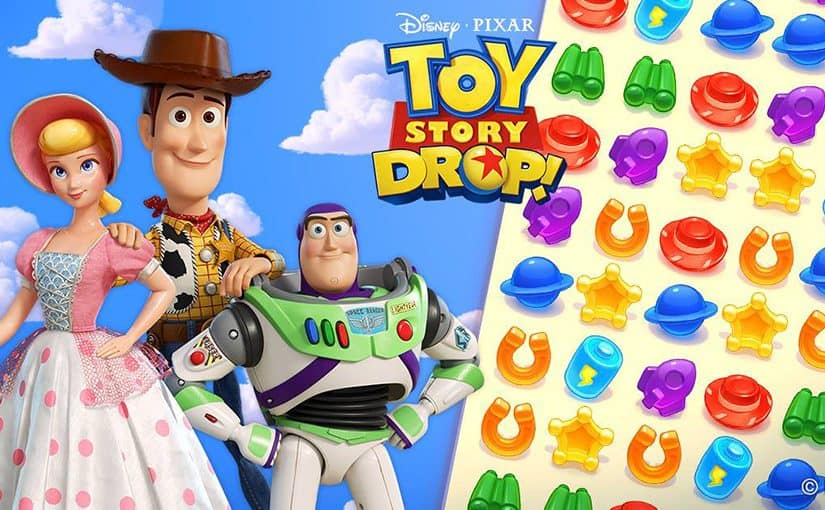
\includegraphics[scale=0.15]{TSD.jpg}
                \end{subfigure}
                \begin{subfigure}{\linewidth}
                    \centering
                    
\includegraphics[scale=0.260]{GD.jpg}
                \end{subfigure}
            \end{subfigure}
        \end{figure}
    \end{frame}
    \begin{frame}
        \frametitle{Игровой движок Citrus}
        \begin{figure}
            \centering
            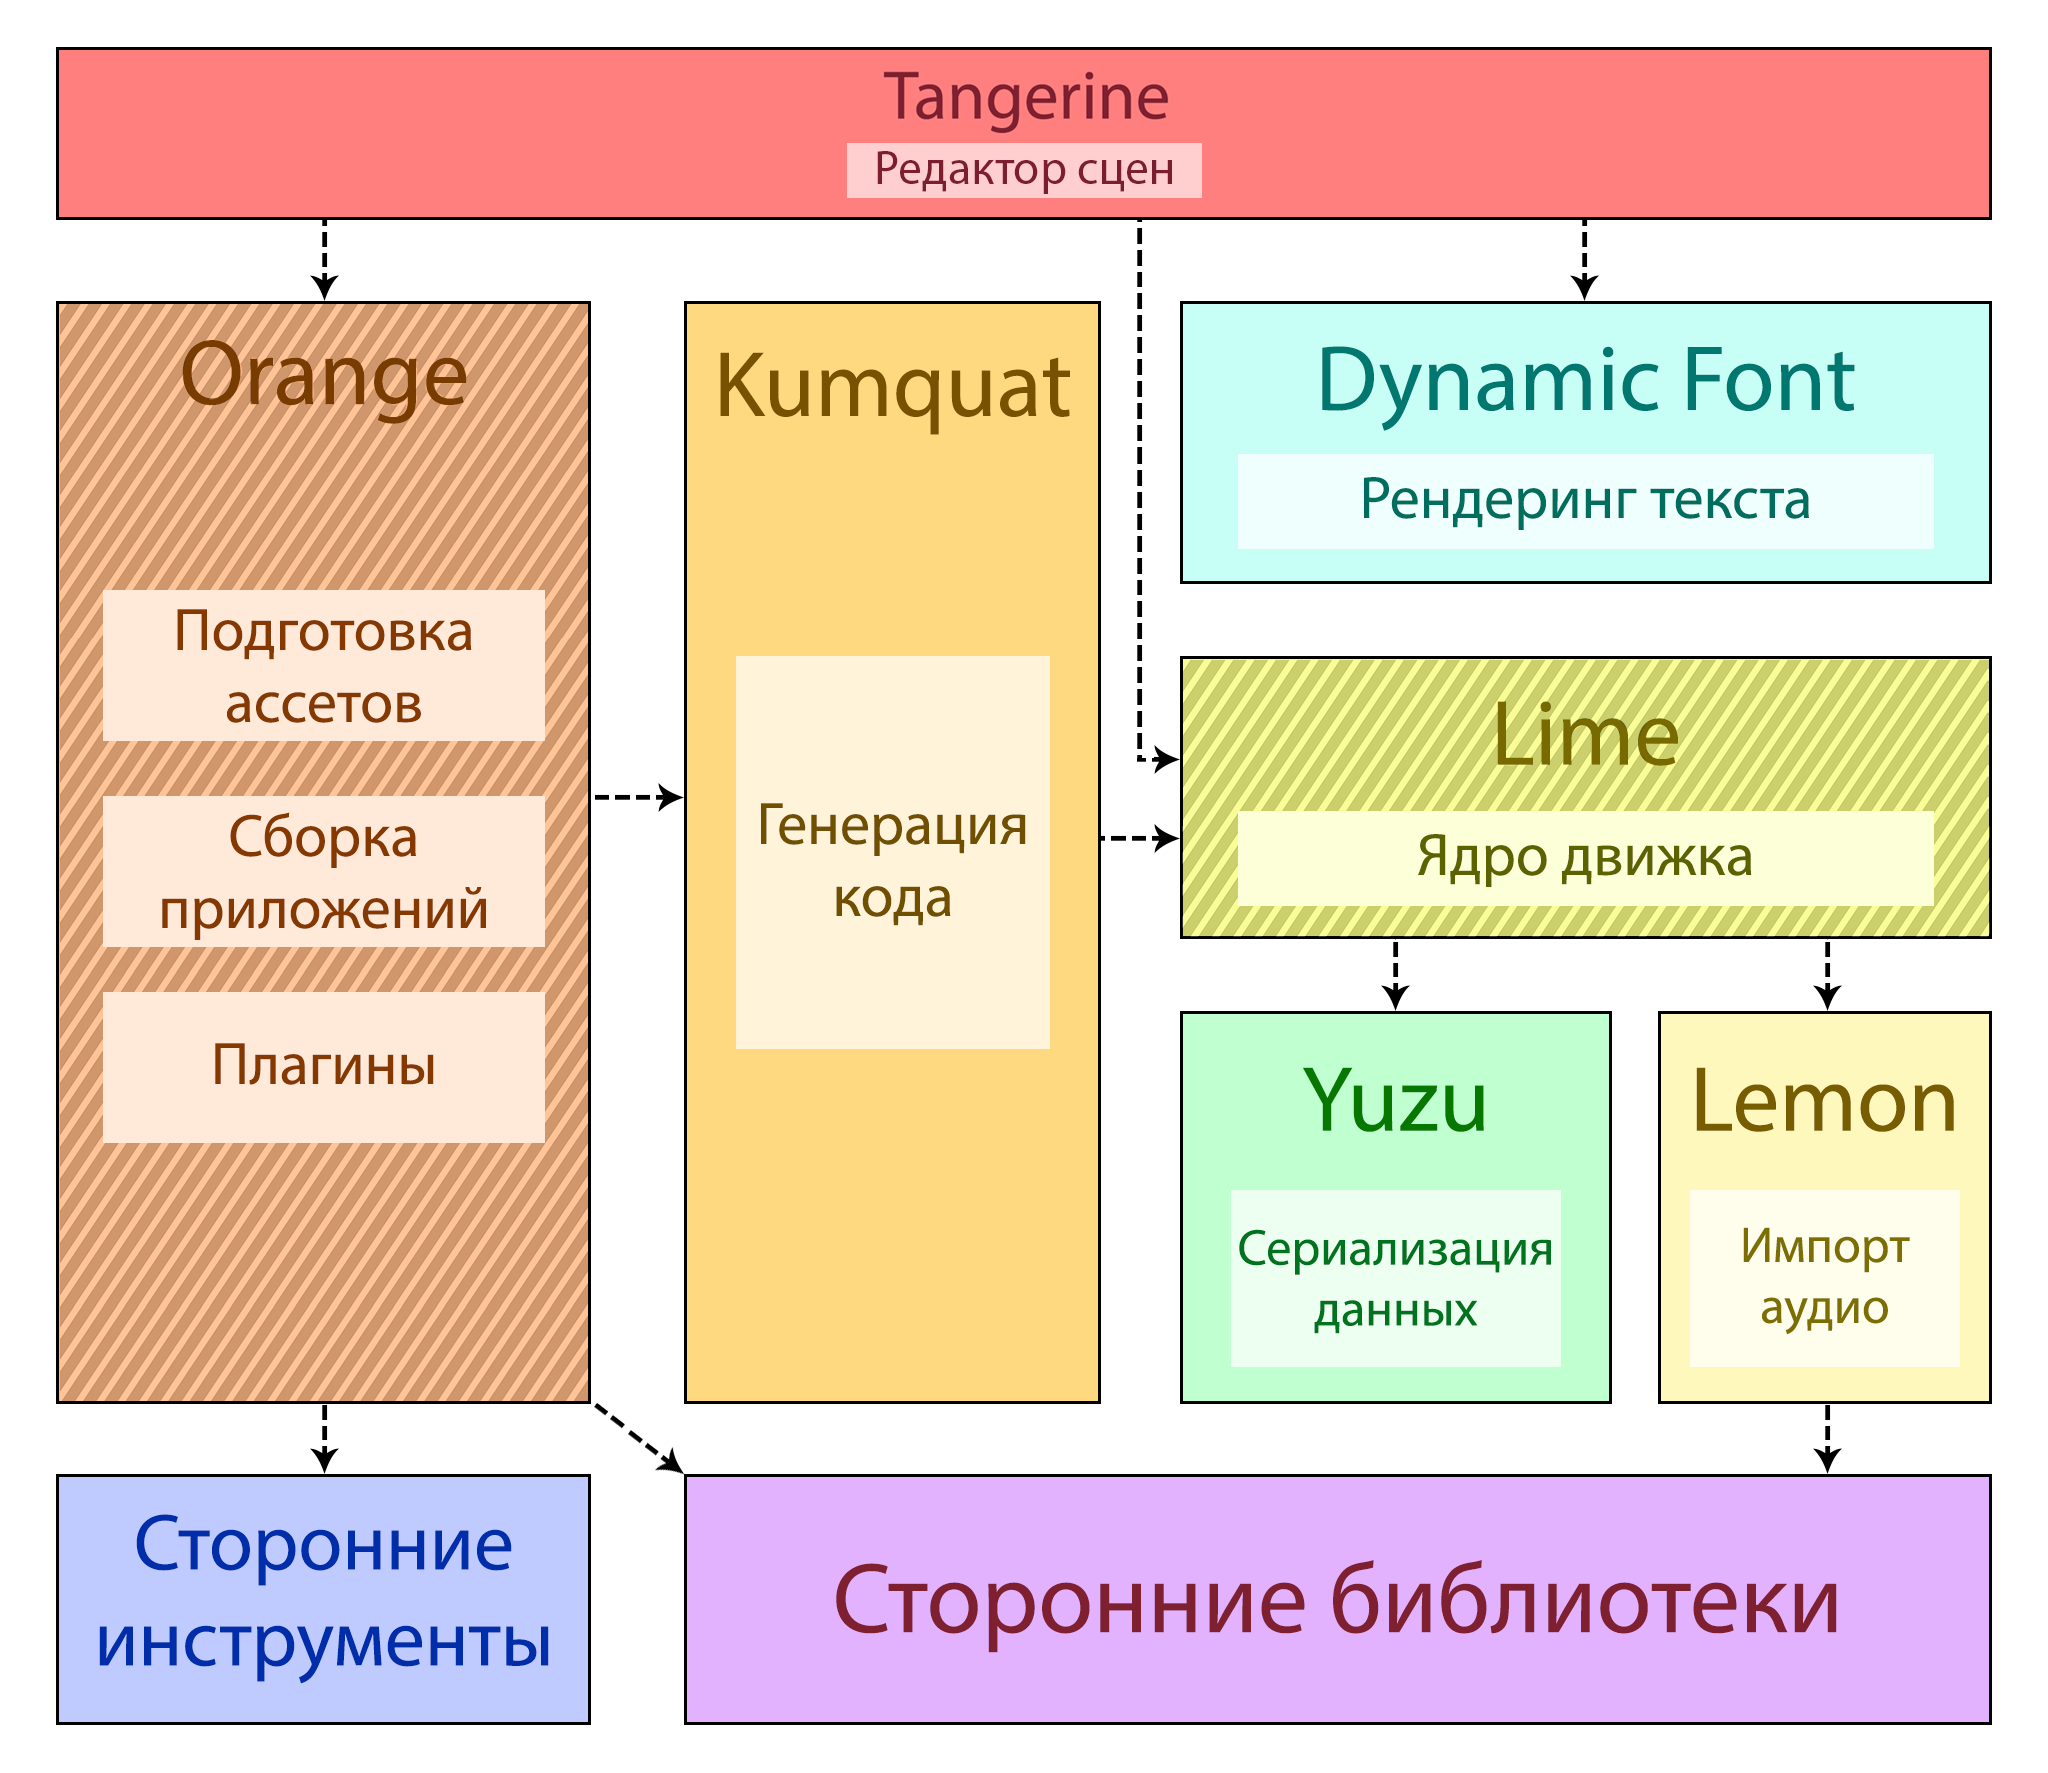
\includegraphics[width=\linewidth, height=.9\textheight, keepaspectratio]{CitrusArchitecture.png}
        \end{figure}
    \end{frame}
    \begin{frame}
        \frametitle{Упаковка текстур в атлас}
        \begin{itemize}
            \item Жадный алгоритм
            \item Генерация текстурного меша, полигональная упаковка методами машинного обучения
        \end{itemize}
        \begin{figure}
            \centering
            \begin{subfigure}[H]{\linewidth}
                \centering
                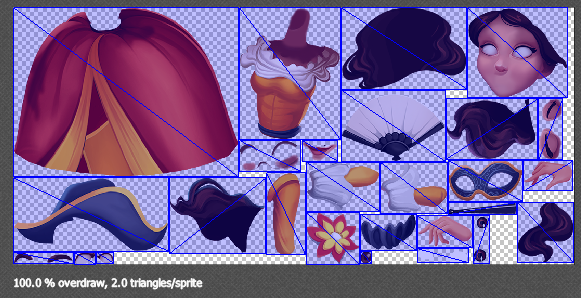
\includegraphics[width=.59\linewidth]{RectangularPacking.png}
            \end{subfigure}
            \vskip .5cm
            \begin{subfigure}[H]{\linewidth}
                \centering
                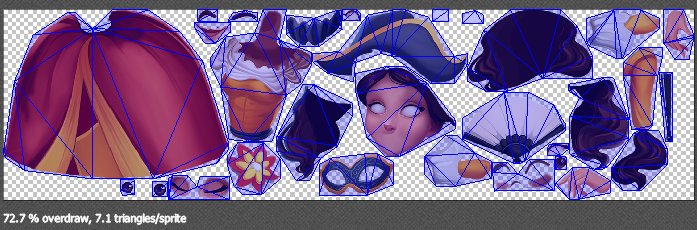
\includegraphics[width=.59\linewidth]{PolygonalPacking.png}
            \end{subfigure}
        \end{figure}
    \end{frame}
    \begin{frame}
        \frametitle{Цели и задачи}
        Цель: оптимизировать отрисовку в играх (уменьшить overdraw, pixel shader invocations и количество разрыва батчей) и уменьшить размер бандла

        Задачи:
        \begin{itemize}
            \item Разработать алгоритм полигонизации текстур
            \item Разработать алгоритм упаковки полигональных текстур в атлас
        \end{itemize}
    \end{frame}
    \begin{frame}
        \frametitle{Этапы полигональной упаковки в атлас}
        \begin{itemize}
            \item Трассировка контура
            \item Аппроксимация контура
            \item Генерация меша
            \item Упаковка в атлас
        \end{itemize}
    \end{frame}
    \begin{frame}
        \frametitle{Трассировка контура}
        Алгоритм Suzuki Satoshi\cite{SuzukiAlgorithm}
        \begin{figure}[H]
            \centering
            \begin{subfigure}[l]{0.50\linewidth}
                \centering
                
\includegraphics[scale=2]{donutpixel_contour_none.png}
            \end{subfigure}
            \begin{subfigure}{0.49\linewidth}
                \centering
                
\includegraphics[scale=2]{donutpixel_contour_simple.png}
            \end{subfigure}
        \end{figure}
    \end{frame}
    \begin{frame}
        \frametitle{Аппроксимация контура}
        Стадии аппроксимации:
        \begin{itemize}
            \item Применение минимальных валидных преобразований
            \item Мердж полигонов
            \item Удаление дыр
            \item Растяжение по фрейму
        \end{itemize}
        \begin{figure}[H]
            \centering
            \begin{subfigure}[l]{0.33\linewidth}
                \centering
                
\includegraphics[scale=1.5]{donutpixel_approx_start.png}
            \end{subfigure}
            \begin{subfigure}{0.33\linewidth}
                \centering
                
\includegraphics[scale=1.5]{donutpixel_approx_mid.png}
            \end{subfigure}\begin{subfigure}{0.33\linewidth}
                \centering
                
\includegraphics[scale=1.5]{donutpixel_approx_end.png}
            \end{subfigure}
        \end{figure}
    \end{frame}
    \begin{frame}
        \frametitle{Аппроксимация контура. Типы преобразований}
        \begin{itemize}
            \item Удаление вогнутого угла для границы или выпуклого для дырки
            \item Замена вершины пересечением двух сторон
            \item Удаление треугольной дырки
        \end{itemize}
        \begin{figure}[H]
            \centering
            \begin{subfigure}[H]{\linewidth}
                \centering
                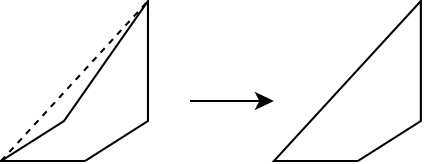
\includegraphics[scale=0.9]{images/convex_angle.png}
                \caption{Удаление вогнутого угла}
            \end{subfigure}
            \vskip .5cm
            \begin{subfigure}[H]{\linewidth}
                \centering
                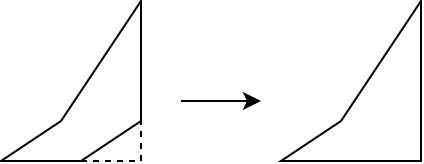
\includegraphics[scale=0.9]{images/sides_intersection.png}
                \caption{Пересечение 2 сторон}
            \end{subfigure}
        \end{figure}
    \end{frame}
    \begin{frame}
        \frametitle{Аппроксимация контура. Детали реализации}
        Триангуляция Делоне\cite{Delaunay} -- бекенд для всех операций
        \begin{figure}[H]
            \centering
            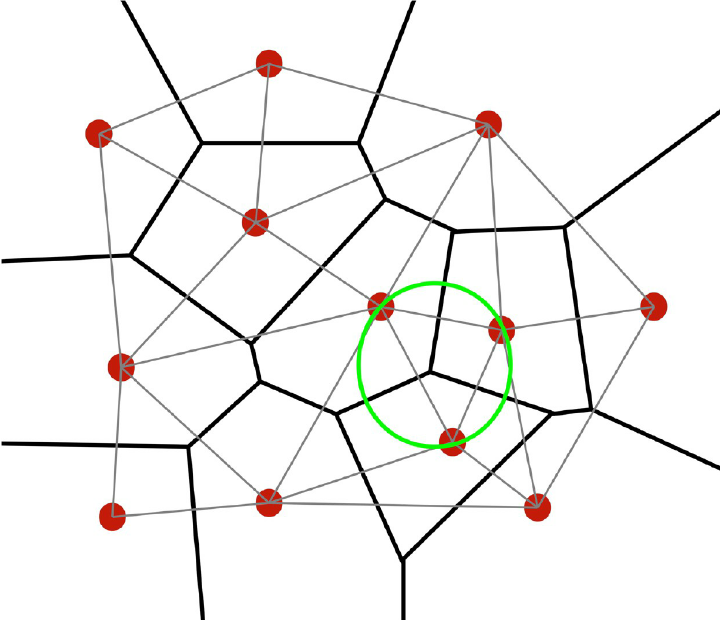
\includegraphics[width=0.7\linewidth, keepaspectratio]{DelaunayAndVoronoi.png}
        \end{figure}
    \end{frame}
    \begin{frame}
        \frametitle{Генерация меша}
        Winding number (non-zero filling rule)
        \begin{figure}[H]
            \centering
            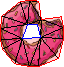
\includegraphics[scale=1.5]{donutpixel_mesh.png}
        \end{figure}
    \end{frame}
    \begin{frame}
        \frametitle{Упаковка в атлас}
        Генетический алгоритм с локальным поиском (memetic algorithm)
        Методы локального поиска:
        \begin{itemize}
            \item Вставить полигон в пустое место
            \item Вставить полигон в дырку
            \item Физика
        \end{itemize}
    \end{frame}
    \begin{frame}
        \frametitle{Упаковка в атлас}
        \begin{figure}
            \centering
            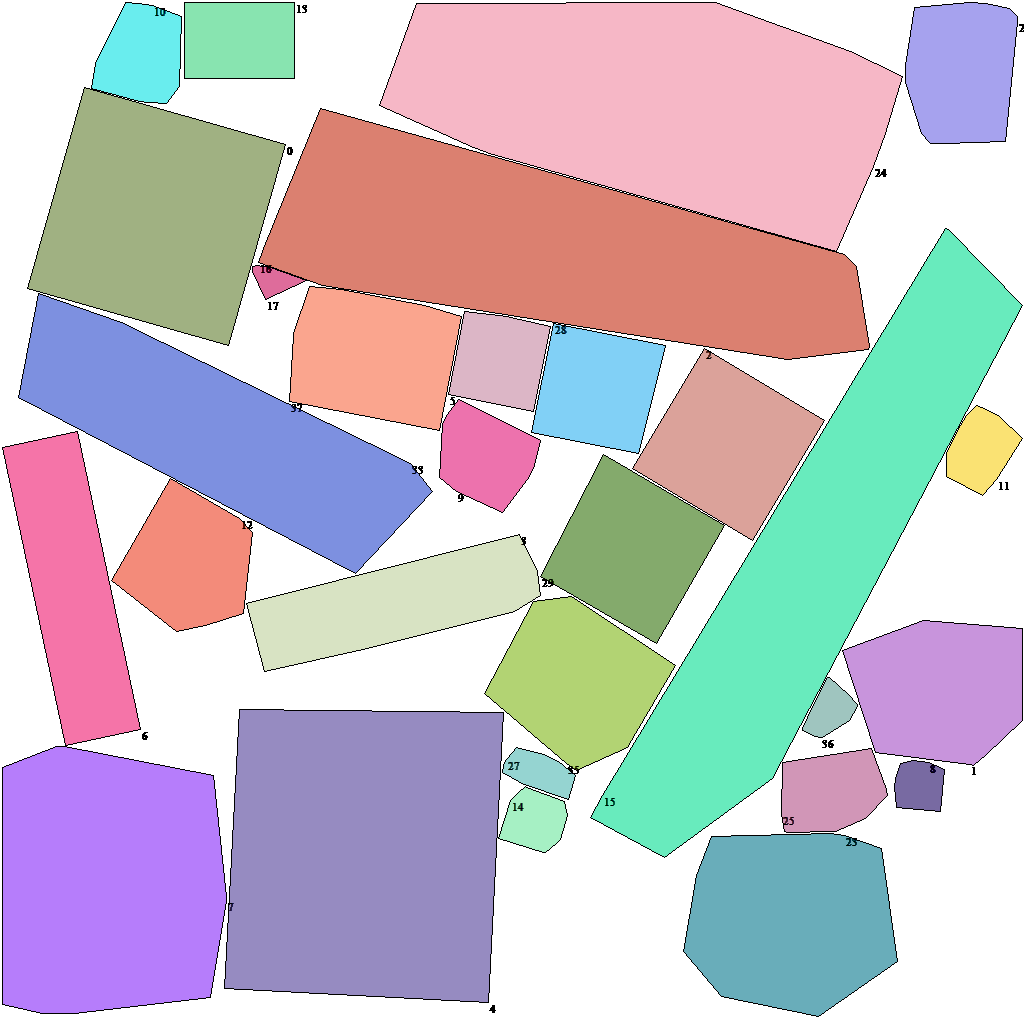
\includegraphics[width=\linewidth, height=.9\textheight, keepaspectratio]{PackExample.png}
        \end{figure}
    \end{frame}
    \begin{frame}
        \frametitle{Оставшаяся часть работы}
        \begin{itemize}
            \item Интеграция в Citrus (в процессе)
            \item Выработать критерий остановки аппроксимации
            \item Разработать алгоритм подбора оптимального размера атласа
        \end{itemize}
    \end{frame}
    \begin{frame} %[allowframebreaks]
        \frametitle{Список литературы}
        \bibliographystyle{ugost2008ls}
        \bibliography{references}
    \end{frame}
\end{document}
